\documentclass[11pt]{article}
\usepackage{latexsym}
\usepackage{amsmath}
\usepackage{amssymb}
\usepackage{amsthm}
\usepackage{epsfig}
\usepackage[tight]{subfigure}

\usepackage{xcolor}
\usepackage{amsmath}

\DeclareMathOperator*{\minimize}{min}
\DeclareMathOperator*{\maximize}{max}

\usepackage{algorithm}
 %on linux you may need to run sudo apt-get install texlive-full to install algorithm.sys
\usepackage{algorithmic}

\usepackage{verbatim}

\newcommand{\handout}[5]{
  \noindent
  \begin{center}
  \framebox{
    \vbox{
      \hbox to 5.78in { {#1} \hfill #2 }
      \vspace{4mm}
      \hbox to 5.78in { {\Large \hfill #5  \hfill} }
      \vspace{2mm}
      \hbox to 5.78in { {\em #3 \hfill #4} }
    }
  }
  \end{center}
  \vspace*{4mm}
}

\newcommand{\lecture}[5]{\handout{#1}{#2}{#3}{#4}{#5}}
\newcommand{\collision}[0]{\mathrm{collision}}
\newcommand{\nocollision}[0]{\overline{\collision}}

\newcommand*{\QED}{\hfill\ensuremath{\square}}

\newtheorem{theorem}{Theorem}
\newtheorem{corollary}[theorem]{Corollary}
\newtheorem{lemma}[theorem]{Lemma}
\newtheorem{observation}[theorem]{Observation}
\newtheorem{proposition}[theorem]{Proposition}
\newtheorem{definition}[theorem]{Definition}
\newtheorem{claim}[theorem]{Claim}
\newtheorem{fact}[theorem]{Fact}
\newtheorem{assumption}[theorem]{Assumption}
\newtheorem{note}[theorem]{Note}

% 1-inch margins, from fullpage.sty by H.Partl, Version 2, Dec. 15, 1988.
\topmargin 0pt
\advance \topmargin by -\headheight
\advance \topmargin by -\headsep
\textheight 8.9in
\oddsidemargin 0pt
\evensidemargin \oddsidemargin
\marginparwidth 0.5in
\textwidth 6.5in

\parindent 0in
\parskip 1.5ex
%\renewcommand{\baselinestretch}{1.25}

\begin{document}

\lecture{Statistical Techniques in Robotics (16-831, S20)}{Lecture \#017
  (Wednesday, March 23)}{Lecturer: Kris Kitani}{Scribes: Shane Deng, Jonathan Schwartz}{Model-Free Value Prediction}



\section{Review}

\subsection{Model-Free vs Model-Based Prediction}

In the last lectures we discussed the two main kinds of Value-based Control: Model-Free and Model-Based. In Model-Based control, you have a model of your environment with the state dynamics and reward function fully specified. 

\begin{figure}[H]
    \centering
    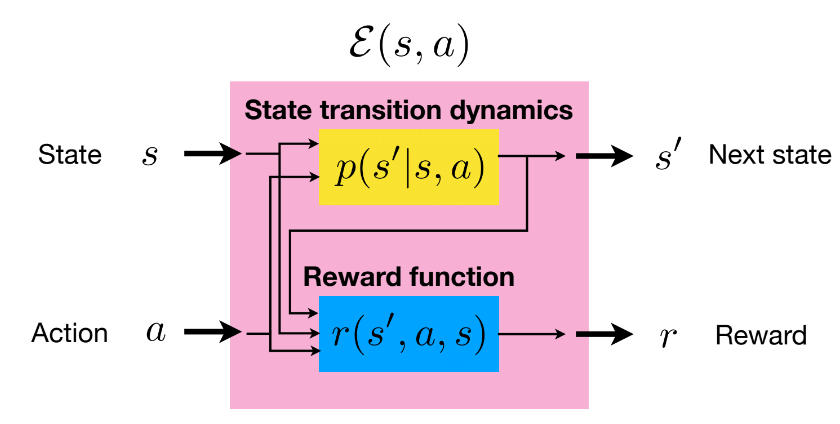
\includegraphics[width=0.35\linewidth]{images/known_model_env.png}
    \caption{Environment where the model is known}
    \label{fig:known_model_env}
\end{figure}

This means you can compute the next step and reward without interacting with the system, which allows you to directly solve for the optimal value function. If you are given a fully specified joint state-reward transition model $p(s', r|s,a)$, you can solve for the state transition dynamic by marginalizing out the reward like so:

\begin{equation}
    p(s' | s,a) = \sum\limits_r{p(s', r|s,a)}
\end{equation}

This gives you everything you need to solve for the reward function given the current state, an action, and the next state:

\begin{equation}
    \mathbb{E}_p[r^{(t)} | s^{(t+1)} = s', a^{(t)}=a, s^{(t)}=s] = \sum\limits_r r \cdot \frac{p(r,s'|s,a)}{p(s'|s,a)} = r(s',a,s)
\end{equation}

You can also solve for the reward function given the current state and action:

\begin{equation}
    \mathbb{E}_p[r^{(t)} | a^{(t)}=a, s^{(t)}=s] = \sum\limits_{r, s'} r \cdot p(r,s'|s,a) = r(a,s)
\end{equation}

For Model-Free Prediction, you do not have direct access to the state dynamics or reward function. This means you must derive information from interacting with the model. We explored the Monte-Carlo and Temporal Difference Prediction methods as approaches to working in these sorts of environments. 

\subsection{Monte-Carlo Prediction}

Monte-Carlo Prediction estimates the value function by interacting with the environment many times. There are several variations of this approach:

\textbf{First-Visit MC Prediction} averages the reward from the first visit to a state to the end of an episode as it follows a policy. It estimates the value function at each state $V(s)$ to equal the average reward from following the policy after these initial visits. 

\textbf{First-Visit Incremental MC Prediction} uses a similar approach, but it uses an incremental update approach where it adjusts the value function in the direction of each first-visit to end of episode reward. It also inversely scales these adjustments with how many visits to the state there have been. This means the rewards from later episodes will not have as large an impact as earlier episodes.

\textbf{Every-Visit MC Prediction} is like First-Visit Incremental MC, with two key differences. The first is that the value function is updated every time a state is reached; not just the first time. The second is that the updates are all scaled by a constant $\alpha$, as opposed to adjusting the scaling factor with the number of prior visits to that state.

These algorithms can be found in the scribe notes and lecture slides for Lecture 16.


\subsection{Temporal Difference Prediction}

Temporal Difference (TD) Prediction also learns by interacting with the environment, but it also uses the idea of "bootstrapping" from dynamic programming to incrementally estimate values after every action. It does this by updating the value function with the immediate reward plus the expected reward at the next state, as opposed to the sum of rewards from the current state to the end of the episode. 

\textbf{MC Reward Approximation:} 

\begin{equation}
    \sum\limits_{i=t}^T r(i)\label{eq:MC_reward}
\end{equation}

\textbf{TD Reward Approximation:} 

\begin{equation}
    r^{(t)} + \gamma V(s^{(t+1)})\label{eq:TD_reward}
\end{equation}

The above expression is for 1-Step TD Prediction. 2-Step TD Prediction uses the same reward approximation, but it adds the term: $\gamma^2 V(s^{(t+2)})$. N-Step TD Prediction uses the same reward approximation, but has terms for the value of the next N states, where the term for state n is: $\gamma^n V(s^{(t+n)})$. TD Prediction uses these reward approximations to update the value function in the same way Every-Visit MC does. It scales the difference in observed value with the current value function by a user-specified constant $\alpha$, and adds it to the value function element corresponding with the current state. 

Details on the different TD Prediction algorithms discussed above can be found in the scribe notes and lecture slides for Lecture 16.

Some of the key points include:
\begin{enumerate}
  \item MC reward updates offline while TD reward updates online
  \item Since the whole trajectory is sampled by the MC algorithm, it accrues high variance. On the contrary, TD algorithm only looks several steps ahead so the variance is lower
  \item MC reward uses unbiased estimator while TD reward uses biased estimator
\end{enumerate}

%This section serves as a review of the previous lecture and any other context required to frame the content of the current lecture. 

%You may format the scribes in any way you like, aside from changing font style, size and page format. Please use subsections and paragraphs to increase the readability of your notes.

%Length requirement 1-2 pages.


\section{Summary}
Some of the key points about TD prediction:
\begin{itemize}
  \item TD prediction works for model-free problems (they can be also used for model-based problems) \textcolor{red}{Note: Sometimes even when we have a model, we still want to use the model-free method in order to solve the problem}
  \item Uses bootstrapping to estimate the value function. a bootstrapping method is essentially computing the estimated value function based on another estimated value function. Note that MC algorithm does not use bootstrapping because they have the model and hence they can compute the value function for the entire trajectory. 
  \item Estimate is biased (due to bootstrapping), low variance as we have discussed before
  \item TD prediction works for infinity horizon problem
\end{itemize}

For N-step TD algorithm, just like 1-step TD and 2-step TD,  we need to specify the step size. In this case, we need to define N. A way to resolve this is TD($\lambda$)
\subsection{$\lambda$-Return Prediction}

Extending equation \ref{eq:TD_reward} to the case where we look N steps into the future gives:
\begin{center}\begin{large}
    $G^{(t)}(N) = r^{(t)}_\gamma r^{(t+1)} + ... + \gamma^{(N-1)}r^{(t+N-1)} + \gamma^N V(s^{(t+N)})$
\end{large}\end{center}

This helps us to derive the Infinite horizon $\lambda$-return algorithm, which predicts the value of the reward $G_{\lambda}^{(t)}$ with a weighted sum of different step TD Reward approximations:

\begin{equation}
    G_{\lambda}^{(t)} =  (1 - \lambda) \sum\limits_{n=1}^\infty \lambda^{(n-1)} G^{(t)}(n)
\end{equation}
$G_{\lambda}^{(t)}$ is the lambda return. $\lambda$ is the trace decay factor. $G^{(t)}(n)$ is the n-step TD target.

The weighting scheme applies smaller weights to larger horizon reward estimates, and is depicted in Figure \ref{fig:lambda-return_weighting} below:

\begin{figure}[H]
    \centering
    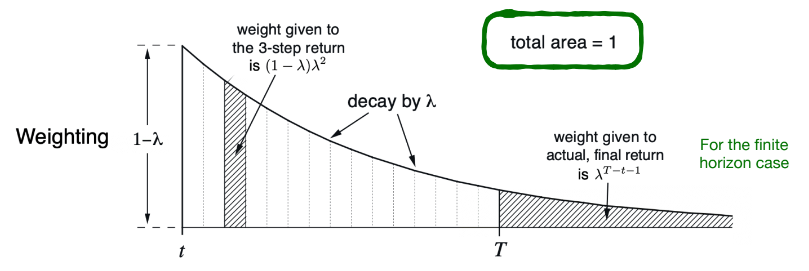
\includegraphics[width=0.35\linewidth]{images/lambda-return_weighting.png}
    \caption{Environment where the model is known}
    \label{fig:lambda-return_weighting}
\end{figure}

There is also a finite horizon version of the algorithm, since infinite sums are impossible to calculate in practice:

\begin{equation}
    G_{\lambda}^{(t)} =  (1 - \lambda) \sum\limits_{n=1}^{T-t-1} \lambda^{(n-1)} G^{(t)}(n) + \lambda^{T-t-1}G^{(t)}(T-t-1)
\end{equation}

To better understand this lambda return function, we can consider two scenarios: \\ 
When $\lambda = 1$:
\begin{center}\begin{large}
    $G_{\lambda}^{(t)} =  G^{(t)}(T-t-1)$
\end{large}\end{center}
This is essentially Monte Carlo estimate of return defined in Equation \ref{eq:MC_reward}. 

When $\lambda = 0$:

\begin{center}\begin{large}
$G_{\lambda}^{(t)} = \sum\limits_{n=1}^{T-t-1} \lambda^{(n-1)} G^{(t)}(n)$
\end{large}\end{center}
This is n-step TD estimate of return.

The Offline $\lambda$-Return algorithm is as follows:

\begin{algorithm}[H]
\caption{Offline-$\lambda$-Return}
\label{algo:OLR}
\begin{algorithmic}[1]
\FOR{$e=1,\;\cdots,\;E$}
\STATE $\{s^{(t)}, a^{(t)}, r^{(t)}\}_{t=0}^T ~ \mathcal{E}|\pi$ \hfill $\triangleright$ sample full episode
\FOR{$t=0,\;\cdots,\;T$} 
\STATE $G_{\lambda}^{(t)} \xleftarrow{} (1 - \lambda) \sum_{n=1}^{\infty} \lambda^{n-1} G^{(t)}(n)$ \hfill $\triangleright$ Precompute all of the returns
\ENDFOR
\FOR{$t=0,\;\cdots,\;T$} 
\STATE $V(s^{(t)} \xleftarrow{} V(s^{(t)}) + \alpha [G_{\lambda}^{(t)} - V(s^{(t)})]$ \hfill $\triangleright$ update value function after episode
\ENDFOR
\ENDFOR
\RETURN V(s)
\end{algorithmic}
\end{algorithm}

Similarly to the n-step TD algorithm, the optimal $\alpha$ is related to the choice of the algorithm's other parameter, $\lambda$. The relationship can be seen in Figure \ref{fig:lambda-return_params} below:

\begin{figure}[H]
    \centering
    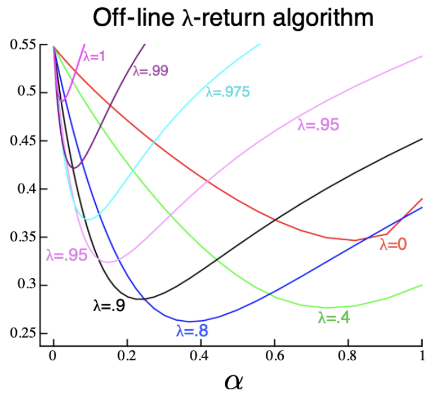
\includegraphics[width=0.35\linewidth]{images/lambda-return_params.png}
    \caption{$\lambda$-return parameters}
    \label{fig:lambda-return_params}
\end{figure}

While offline $\lambda$-return is useful to understand the general $\lambda$-return function, it is not particularly practical. This is because it cannot be implemented online, since you need the full future trajectory at each time step in order to update the value function. At the same time, when compared to n-step TD, the performance of off-line lambda return only performs slightly better. 

Combining $\lambda$-return with the TD algorithms we have explored previously produces a useful algorithm that can be used online. To do so, we need to use eligibility traces. 

\subsection{TD($\lambda$) Prediction}

Before we get into the TD($\lambda$) algorithm, we will derive an expression for the TD error that shows it can be expressed as a sum of weighted one step TD errors.

\begin{large}
    \textbf{Starting with the definition of a $\lambda$-return:}\\\vspace{1mm}
    $\Delta V(s^{(t)}) = G_{\lambda}^{(t)} - V(s^{(t)})$\\
    $\null\;\,\Delta V(s^{(t)}) = (1 - \lambda) \sum\limits_{n=1}^{\infty} \lambda^{n-1} G_{\lambda}^{(t)} - V(s^{(t)})$
    
    \textbf{Expand the sum using Equation \ref{eq:TD_reward}:}\\\vspace{1mm}
    $\Delta V(s^{(t)}) = (1 - \lambda) [\lambda^0 G^{(t)}(1) + \lambda^1 G^{(t)}(2) + \lambda^2 G^{(t)}(3)+\cdots] - V(s^{(t)})$
    
    \textbf{Separate out n-step TD targets:}\\\vspace{1mm}
    $\Delta V(s^{(t)}) = (1 - \lambda) \lambda^0 (r^{(t)} + \gamma V(s^{(t+1)})) - V(s^{(t)})$\\
    $\null \hspace{15mm} + (1 - \lambda) \lambda^1 (r^{(t)} + \gamma r^{(t+1)} + \gamma^2 V(s^{(t+2)}))$\\
    $\null \hspace{15mm} + (1 - \lambda) \lambda^2 (r^{(t)} + \gamma r^{(t+1)} + \gamma^2 r^{(t+2)} + \gamma^3 V(s^{(t+3)}))$\\
    $\null \hspace{15mm} + \cdots$
    
    \textbf{Multiplying out the $(1-\lambda)$ terms (red terms will cancel out):}\\\vspace{1mm}
    $\Delta V(s^{(t)}) = \lambda^0 (r^{(t)} + \gamma V(s^{(t+1)})) - \lambda^1 (\textcolor{red}{r^{(t)}} + \gamma V(s^{(t+1)})) - V(s^{(t)})$\\
    $\null \hspace{15mm} + \lambda^1 (\textcolor{red}{r^{(t)}} + \gamma r^{(t+1)} + \gamma^2 V(s^{(t+2)})) - \lambda^2 (\textcolor{red}{r^{(t)} + \gamma r^{(t+1)}} + \gamma^2 V(s^{(t+2)}))$\\
    $\null \hspace{15mm} + \lambda^2 (\textcolor{red}{r^{(t)} + \gamma r^{(t+1)}} + \gamma^2 r^{(t+2)} + \gamma^3 V(s^{(t+3)})) - \lambda^3 (r^{(t)} + \gamma r^{(t+1)} + \gamma^2 r^{(t+2)} + \gamma^3 V(s^{(t+3)}))$\\
    $\null \hspace{15mm} + \cdots$
    
    \textbf{Removing cancelled terms and collecting like terms:}\\\vspace{1mm}
    $\Delta V(s^{(t)}) = (\gamma \lambda)^0 (r^{(t)} + \gamma V(s^{(t+1)})) -  \gamma \lambda V(s^{(t+1)})) - V(s^{(t)})$\\
    $\null \hspace{15mm} + (\gamma \lambda)^1 (r^{(t+1)} + \gamma V(s^{(t+2)}) - \gamma \lambda V(s^{(t+2)}))$\\
    $\null \hspace{15mm} + (\gamma \lambda)^2 (r^{(t+2)} + \gamma V(s^{(t+3)}) - \gamma \lambda V(s^{(t+3)}))$\\
    $\null \hspace{15mm} + \cdots$
    
    \textbf{Which reduces to the sum of 1-step TD errors:}\\\vspace{1mm}
    $\Delta V(s^{(t)}) = (\gamma \lambda)^0 \delta^{(t)} + (\gamma \lambda)^1 \delta^{(t+1)} + (\gamma \lambda)^2 \delta^{(t+2)} + \cdots$\\
    $\null\;\,\Delta V(s^{(t)}) = \sum\limits_{i=0}^\infty (\gamma \lambda)^{i} \delta^{(t+i)}$
    
    \textbf{When $s^{(k)} = s$ (i.e. the last occurrence of state s at time step k):}\\\vspace{1mm}
    $\Delta V(s^{(t)}) = \sum\limits_{t=k}^\infty (\gamma \lambda)^{t-k} \delta^{(t)}$
\end{large}

Thus, we have shown that the TD-lambda error at time step k for state s can be expressed as a decaying weighted sum of future 1-step TD errors.

\begin{large}
    \textbf{Deriving a more concise expression:}
    \begin{equation}
    \sum\limits_{t=k}^\infty (\gamma \lambda)^{t-k} \delta^{(t)} = \sum\limits_{t=1}^{k-1} (0) \delta^{(t)} + \sum\limits_{t=k}^{\infty} (\gamma \delta)^{(t-k)} \delta^{(t)} = \sum\limits_{t=1}^{\infty} z^{(t)}(s) \delta^{(t)}
    \end{equation}
    
    \begin{center}
    $z^{(t)}(s) = \begin{cases} 
      0 & t < k \\
      (\gamma \lambda)^{(t-k)} & t \geq k 
     \end{cases}$
    \end{center}
\end{large}

This weighting function $z^{(t)}(s)$ is called the \textbf{eligibility trace}.

The eligibility trace can also be rewritten into a form with incremental update:\\
\begin{equation}
    z^{(t)}(s) = \gamma \lambda z^{(t-1)}(s) + 1[s^{(t)} = s]
\end{equation}

Note that these two functions are not exactly identical. For the original function, the value can't go over 1 because of the piece-wise functions. For the new incremental form, $z^{(t)}(s)$ can be larger than 1.
\begin{figure}[H]
    \centering
    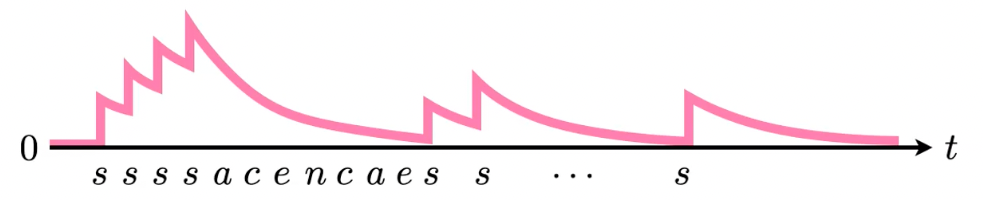
\includegraphics[width=0.5\linewidth]{images/Eligibility Trace.png}
    \caption{Eligibility Trace}
    \label{fig:lambda-return_params}
\end{figure}

The eligibility trace is essentially the memory of the algorithm. In the function, $\gamma \lambda Z^{(t-1)}(s)$ is the decay of the current state. In other words, if the state is very distant or seen long time ago, then it will decay. In the example, starting in state a, the algorithm hasn't seen state s for a long time then the value decreases quickly. For the second term in the function $1[s^{(t)} = s]$, the indicator function turns on when the same state repeats. In other words, this tracks how many times the same state has repeated. 

We can rewrite the offline update equation by using eligibility trace in algorithm \ref{algo:OLR}:

$$V(s^{(t)}) = V(s^{(t)}) + \alpha [G_{\lambda}^{(t)} - V(s^{(t)})]$$ Which can be simplified to: 
\begin{equation}
V(s) = V(s) + \sum_{i=0}^\infty \alpha z^{(i)} \delta
\end{equation}

Then we can substitute $Z(s)$ with the new incremental update equation, which will allow the function to be updated incrementally at every step. This then turns into online update since we can update at every step:

\begin{equation}
V(s) = V(s) + \alpha z \delta
\end{equation}

\begin{equation}
V(s) = V(s) + \alpha z(s) [r^{(t)} + \gamma V(s^{(t+1)}) - V(s^{(t)})]
\end{equation}

\begin{algorithm}[H]
\caption{TD($\lambda$)-prediction}
\label{algo:TDP}
\begin{algorithmic}[1]
\FOR{$t=1,\;\cdots,\;T$}
\STATE $\{s^{(t+1)}, a^{(t)}, r^{(t)}\}_{t=0}^T ~ \mathcal{E}|\pi,s^{(t)}$ \hfill $\triangleright$ select action, get reward, then go to next state
\STATE $\delta \xleftarrow{} r^{(t)} + \gamma V(s^{(t+1)}) - V(s^{(t)})$ \hfill $\triangleright$ Compute 1-step TD error
\FOR{$s \in S$} 
\STATE $ z(s) \xleftarrow{} \gamma \lambda Z^(t-1)(s) + 1[s^{(t)} = s]$\hfill $\triangleright$ update eligibility trace
\STATE $V(s) \xleftarrow{} V(s) + \sum_{i=0}^\infty \alpha z^{(i)} \delta$\hfill $\triangleright$ update value function
\ENDFOR
\ENDFOR
\RETURN V(s)
\end{algorithmic}
\end{algorithm}

We can substitute different values for the algorithm to see how the algorithm performs
\begin{center}
\begin{tabular}{||c c||} 
 \hline
 value & algorithm \\ [0.5ex] 
 \hline\hline
 $\lambda = 0$ & One step TD prediction  \\ 
 \hline
 $\lambda < 1$ & TD($\lambda$) \\
 \hline
 $\lambda = 1$ & No Decay, Discounted Monte Carlo prediction \\
 \hline
 $\lambda = 1 \And \gamma = 1$ & No decay, Monte Carlo prediction \\
 \hline
\end{tabular}
\end{center}
\section{Appendix}

\subsection{Monte Carlo}
Much of the previous and this lectures rely on the understanding of Monte Carlo and how it works. In class, we discussed that Monte Carlo is a process of repeated random sampling process. The example we used in class is that we can generate numerous trajectories and we will sample these trajectory to find the most likely trajectory the algorithm is going to select. In this appendix, we are going to discuss Monte Carlo more in depth and its other statistical applications.\\ \\
\begin{figure}[H]
    \centering
    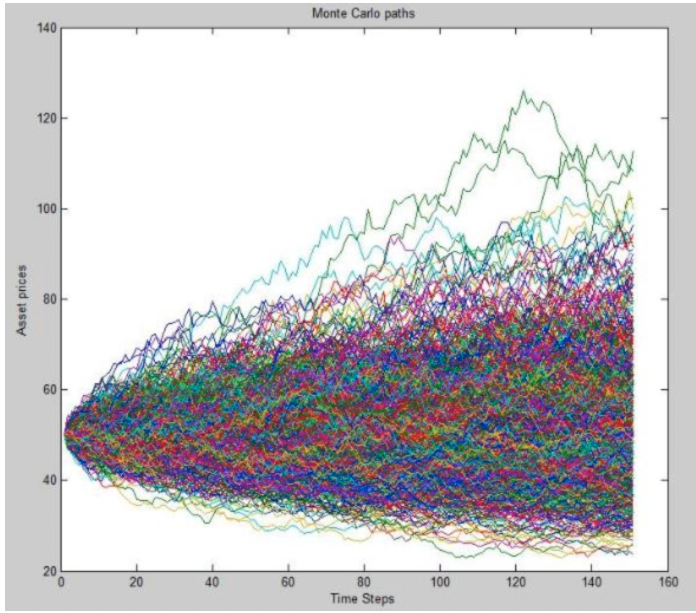
\includegraphics[width=0.35\linewidth]{images/Monte Carlo Sampling .png}
    \caption{Monte Carlo Sampling [4]}
    \label{fig:lambda-return_params}
\end{figure}

First of all, Monte Carlo is a subset of computational algorithms that uses sampling algorithm to estimate unknown parameters. Many modern systems are very complicated and it is nearly impossible to calculate all the parameters accurately. An interesting application of Monte Carlo method is to estimate $\pi$. Assume a rectangle with a circle inside, then the algorithm randomly selects a point in the rectangle. After many samples, then calculate the ratio between the points in the circle and total number of points. By using the area ratio, we can estimate the value of $\pi$ and the value is fairly accurate. Some other applications also include financial market prediction since the financial system can be very complicated.  
\begin{figure}[H]
    \centering
    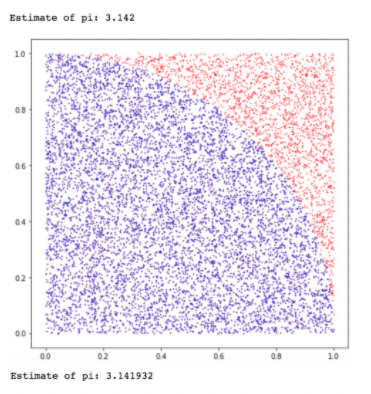
\includegraphics[width=0.35\linewidth]{images/pi estimation.png}
    \caption{Using Monte Carlo to estimate pi [4]}
    \label{fig:lambda-return_params}
\end{figure}

\subsection{Monte Carlo Tree Search}
Monte Carlo Tree Search was used in many AI applications. The most prominent one is google AlphaGO which defeated the human player. Monte Carlo Tree Search Algorithm essentially samples the possible actions to find the most promising action. In computer science, tree search is a general algorithm to search tree-like data structures. However, traditional BFS and DFS algorithms become very time consuming when it comes to complicated systems like GO, which has higher number of possibilities than the number of atoms in the universe. Monte Carlo Tree Search essentially tries to balance the exploration and exploitation. Behind the scene of AlphaGO, a UCB based policy is used. This is similar to the UCB algorithm we learned in the Multi-armed bandit lectures. \\
For every node in the tree:

\begin{equation}
UCB(node_i) = \Bar{x} +C\sqrt{\dfrac{\log{N}}{n}}
\end{equation}
where $\Bar{x}$ is the mean, n is the visits of the node, N is the number of visit parent. This UCB algorithm balances the mean and variance (in this case, the number of nodes visited)

\subsection{Monte Carlo VS Bootstrapping}
In class, we talked about both Monte Carlo as well as Bootstrapping. In the case of model based reinforcement learning, we use MC to sample the trajectories and find the most promising one. In TD, we use bootstrapping to use value function to estimate the value function.\\
Both approaches require re-sampling, so what is the difference between the two? \\
Bootstrapping is to re-sample from known samples whereas Monte Carlo is generating data using known distribution and parameters. For instance, if you have 10 numbers {1,2,3,5,6,8,5,2,3,4}, but we want to better understand the distribution. Then we can re-sample from this distribution many times and plot the mean on a histogram graph. The key term is called sample with replacement. 

\subsection{A similar approach: Jack-Knife Resampling}
Jack-Knife is another re-sampling technique that is heavily used for bias and variance estimation. The idea behind this algorithm is relatively simple, which is basically to calculate the sample mean by sequentially removing one observation from the sample. 

\begin{equation}
\Bar{X}_{jack} = \dfrac{1}{n} \sum_{i=1}^n \dfrac{1}{n-1} \sum_{j\in [n], j\neq i} {x_j}
\end{equation}

For example, if the dataset is x1, x2, x3, during the first time, we calculate the mean for all three. Then during the next iteration, we remove x1, and only calculate x2 and x3, and for the final iteration, we only calculate the mean using x3. Then we calculate the weighted sum of all three means to get the jack-knife value. \\ \\
Note that the key difference between Jack-knife and bootstrap is that bootstrap involves sample with replacement while jack-knife involves sampling without replacement. This difference results in the fact that bootstrap tends to be more computationally intensive. and jack-knife's estimated standard error is likely to be higher than bootstrap sampling 

%\section*{References}
%Include your references here. Please cite any resources you found useful.	
%Populate the refs.bib file or list your references manually. Be consistent in formatting!
{
\bibliography{refs}
\bibliographystyle{abbrv}
[1]McIntosh, A. The Jack knife Estimation Method. Retrieved March 26, 2022 from: http://people.bu.edu/aimcinto/jackknife.pdf
Ramachandran, K. \& Tsokos, C. (2014). Mathematical Statistics with Applications in R. Elsevier.\\

[2]Wang, B. (2021, January 11). Monte Carlo Tree Search: An introduction. Medium. Retrieved March 26, 2022, from https://towardsdatascience.com/monte-carlo-tree-search-an-introduction-503d8c04e168 \\

[3]Lecture note from MIT: $https://ocw.mit.edu/courses/brain-and-cognitive-sciences/9-07-statistics-for-brain-and-cognitive-science-fall-2016/lecture-notes/MIT9_07F16_lec11.pdf$\\

[4] Pease, C. (2018, September 11). An overview of Monte Carlo methods. Medium. Retrieved April 5, 2022, from https://towardsdatascience.com/an-overview-of-monte-carlo-methods-675384eb1694 
}


%\section{Appendix}
%This section provides any relevant background material that was not covered in the lectures, but was found to be useful for understanding the material. 
%For example, derivations, theory underlying techniques employed, etc. 

%Additionally, this section can summarizes applications or extensions of these techniques found in the literature. 


\end{document} % Done!


